%abstract classes%%%%%%%%%%%%%%%%%%%%%%%%%%%%%%%%%%%%%%%%%%%%%%%%%%%%%%%%%%%%%%%%%%%
% Sensorthing<SensorthingT> 
\rule{\textwidth}{0.4pt}
\class{Sensorthing<SensorthingT>}
\begin{minipage}{0.4\textwidth}
    \begin{figure}[H]
        {\centering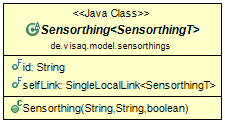
\includegraphics[width=0.95\textwidth]{media/backend/modell/classes/Sensorthing.png}}
    \end{figure}
    \end{minipage} \hfill
    \begin{minipage}{0.6\textwidth}
Die abstrakte Klasse Sensorthing stellt ein Objekt aus der \gls{SensorThings API} da.
Die Klasse vereint die gemeinsamen Eigenschaften der Klassen aus der Datenbank-\gls{API} in sich.
Um die Datentypen der Parameter möglichst exakt zu bestimmen werden \glspl{bounded quantification} verwendet.
\end{minipage}

Attribute:
\begin{itemize}
    \item \emph{public String id} Jedes Objekt der Datenbank-\gls{API} ist mit einer eindeutigen ID versehen, die das Objekt identifiziert.
    Da sich die ID aus Buchstaben, Zeichen und Ziffern zusammensetzt wird sie hier durch einen String repräsentiert.
    \item \emph{public SingleLocalLink<SensorthingT> selfLink} Jedes Objekt der \gls{SensorThings API} hält einen Verweis auf die Online-Instanz von sich selbst.
    So kann die Herkunft und die übereinstimmung des Datensatzes mit der Online-Version jederzeit überprüft werden.
\end{itemize}
Methoden: \begin{itemize}
    \item \emph{public Sensorthing(String id, String selfURL, boolean relative)} Diese Methode ist er einzige Konstruktor der Sensorthing-Klasse.
    Als Parameter erhält der Konstruktor neben dem Klassen-Attribut id auch eine URL und eine boolean relative. Beide Parameter werden zum initialisieren des SingleLocalLink benötigt.
\end{itemize}

%%interfaces%%%%%%%%%%%%%%%%%%%%%%%%%%%%%%%%%%%%%%%%%%%%%%%%%%%%%%%%%%%%%%%%%%%
% SensorthingsProperties
\rule{\textwidth}{0.4pt}
\class{SensorthingsProperties}
\begin{minipage}{0.4\textwidth}
    \begin{figure}[H]
        {\centering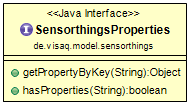
\includegraphics[width=0.95\textwidth]{media/backend/modell/classes/SensorthingsProperties.png}}
    \end{figure}
    \end{minipage} \hfill
\begin{minipage}{0.6\textwidth}
Die Schnittstelle SensorthingsProperties zeigt an, dass ein Objekt der \gls{SensorThings API} Properties besitzt.
Properties sind in diesem Fall Daten vom Typ Object die durch einen String als eindeutigen Identifier gesucht werden können.
Es wird nicht näher spezifiziert welche Properties ein entsprechendes Object muss.
\end{minipage}

Methoden: \begin{itemize}
    \item \emph{public Object getPropertyByKey(String key)} Die Methode sucht in den properties des Objektes eine Eigenschaft mit dem gegebenen Key und gibt den Wert dieser zurück.
    Wenn keine passende Eigenschaft gefunden wurde wird null zurück gegeben.
    \item \emph{public boolean hasProperties(String key)} Die Methode überprüft ob eine Eigenschaft mit dem gegebene Key existiert.
    Falls eine solche Eigenschaft existiert wird true zurück gegeben, andernfalls false.
\end{itemize}

% SensorthingsTimeStamp
\rule{\textwidth}{0.4pt}
\class{SensorthingsTimeStamp}
\begin{minipage}{0.4\textwidth}
    \begin{figure}[H]
        {\centering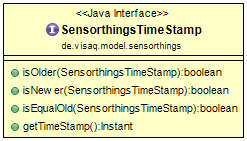
\includegraphics[width=0.95\textwidth]{media/backend/modell/classes/SensorthingsTimeStamp.png}}
    \end{figure}
    \end{minipage} \hfill
\begin{minipage}{0.6\textwidth}
Die Schnittstelle SensorthingsTimeStamp zeigt an, dass ein Objekt der \gls{SensorThings API} einen Zeitstempel besitzt.
Ein Zeitstempel impliziert in diesem Fall, dass zwei solche Objekte anhand ihres Zeitstempels verglichen werden können.
\end{minipage}

Methoden: \begin{itemize}
    \item \emph{public boolean isOlder(SensorthingsTimeStamp other)} Die Methode prüft ob die Instanz älter als die mit other gegebene Instanz ist.
    In diesem Fall wird true zurückgegeben, ansonsten false.
    \item \emph{public boolean isNewer(SensorthingsTimeStamp other)} Die Methode prüft ob die Instanz jünger als die mit other gegebene Instanz ist.
    In diesem Fall wird true zurückgegeben, ansonsten false.
    \item \emph{public boolean isEqualOld(SensorthingsTimeStamp other)} Die Methode prüft ob die Instanz gleich alt wie die mit other gegebene Instanz ist.
    In diesem Fall wird true zurückgegeben, ansonsten false.
    \item \emph{public Instant getTimeStamp()} Die Methode gibt den Zeitstempel als java.time.Instant zurück.
\end{itemize}

%Classes%%%%%%%%%%%%%%%%%%%%%%%%%%%%%%%%%%%%%%%%%%%%%%%%%%%%%%%%%%%%%%%%%%%%%%%
